\documentclass[a4paper]{article}
% * <edvin.wahlberg@gmail.com> 2017-03-20T12:15:45.803Z:
%
% ^.
\usepackage[utf8]{inputenc}

\usepackage[swedish, english]{babel}
\usepackage{amsmath}
\usepackage{graphicx}
\usepackage[colorinlistoftodos]{todonotes}
\usepackage{float}
%code begin
\usepackage{color}
\definecolor{lightgray}{rgb}{0.95, 0.95, 0.95}
\definecolor{darkgray}{rgb}{0.4, 0.4, 0.4}
%\definecolor{purple}{rgb}{0.65, 0.12, 0.82}
\definecolor{editorGray}{rgb}{0.95, 0.95, 0.95}
\definecolor{editorOcher}{rgb}{1, 0.5, 0} % #FF7F00 -> rgb(239, 169, 0)
\definecolor{editorGreen}{rgb}{0, 0.5, 0} % #007C00 -> rgb(0, 124, 0)
\definecolor{orange}{rgb}{1,0.45,0.13}		
\definecolor{olive}{rgb}{0.17,0.59,0.20}
\definecolor{brown}{rgb}{0.69,0.31,0.31}
\definecolor{purple}{rgb}{0.38,0.18,0.81}
\definecolor{lightblue}{rgb}{0.1,0.57,0.7}
\definecolor{lightred}{rgb}{1,0.4,0.5}
\usepackage{upquote}
\usepackage{listings}
% CSS
\lstdefinelanguage{CSS}{
  keywords={color,background-image:,margin,padding,font,weight,display,position,top,left,right,bottom,list,style,border,size,white,space,min,width, transition:, transform:, transition-property, transition-duration, transition-timing-function},	
  sensitive=true,
  morecomment=[l]{//},
  morecomment=[s]{/*}{*/},
  morestring=[b]',
  morestring=[b]",
  alsoletter={:},
  alsodigit={-}
}

% JavaScript
\lstdefinelanguage{JavaScript}{
  morekeywords={typeof, new, true, false, catch, function, return, null, catch, switch, var, if, in, while, do, else, case, break},
  morecomment=[s]{/*}{*/},
  morecomment=[l]//,
  morestring=[b]",
  morestring=[b]'
}

\lstdefinelanguage{HTML5}{
  language=html,
  sensitive=true,	
  alsoletter={<>=-},	
  morecomment=[s]{<!-}{-->},
  tag=[s],
  otherkeywords={
  % General
  >,
  % Standard tags
	<!DOCTYPE,
  </html, <html, <head, <title, </title, <style, </style, <link, </head, <meta, />,
	% body
	</body, <body,
	% Divs
	</div, <div, </div>, 
	% Paragraphs
	</p, <p, </p>,
	% scripts
	</script, <script,
  % More tags...
  <canvas, /canvas>, <svg, <rect, <animateTransform, </rect>, </svg>, <video, <source, <iframe, </iframe>, </video>, <image, </image>, <header, </header, <article, </article
  },
  ndkeywords={
  % General
  =,
  % HTML attributes
  charset=, src=, id=, width=, height=, style=, type=, rel=, href=,
  % SVG attributes
  fill=, attributeName=, begin=, dur=, from=, to=, poster=, controls=, x=, y=, repeatCount=, xlink:href=,
  % properties
  margin:, padding:, background-image:, border:, top:, left:, position:, width:, height:, margin-top:, margin-bottom:, font-size:, line-height:,
	% CSS3 properties
  transform:, -moz-transform:, -webkit-transform:,
  animation:, -webkit-animation:,
  transition:,  transition-duration:, transition-property:, transition-timing-function:,
  }
}

\lstdefinestyle{htmlcssjs} {%
  % General design
%  backgroundcolor=\color{editorGray},
  basicstyle={\footnotesize\ttfamily},   
  frame=b,
  % line-numbers
  xleftmargin={0.75cm},
  numbers=left,
  stepnumber=1,
  firstnumber=1,
  numberfirstline=true,	
  % Code design
  identifierstyle=\color{black},
  keywordstyle=\color{blue}\bfseries,
  ndkeywordstyle=\color{editorGreen}\bfseries,
  stringstyle=\color{editorOcher}\ttfamily,
  commentstyle=\color{brown}\ttfamily,
  % Code
  language=HTML5,
  alsolanguage=JavaScript,
  alsodigit={.:;},	
  tabsize=2,
  showtabs=false,
  showspaces=false,
  showstringspaces=false,
  extendedchars=true,
  breaklines=true,
  % German umlauts
  literate=%
  {Ö}{{\"O}}1
  {Ä}{{\"A}}1
  {Ü}{{\"U}}1
  {ß}{{\ss}}1
  {ü}{{\"u}}1
  {ä}{{\"a}}1
  {ö}{{\"o}}1
}
%
\lstdefinestyle{py} {%
language=python,
literate=%
*{0}{{{\color{lightred}0}}}1
{1}{{{\color{lightred}1}}}1
{2}{{{\color{lightred}2}}}1
{3}{{{\color{lightred}3}}}1
{4}{{{\color{lightred}4}}}1
{5}{{{\color{lightred}5}}}1
{6}{{{\color{lightred}6}}}1
{7}{{{\color{lightred}7}}}1
{8}{{{\color{lightred}8}}}1
{9}{{{\color{lightred}9}}}1,
basicstyle=\footnotesize\ttfamily, % Standardschrift
numbers=left,               % Ort der Zeilennummern
%numberstyle=\tiny,          % Stil der Zeilennummern
%stepnumber=2,               % Abstand zwischen den Zeilennummern
numbersep=5pt,              % Abstand der Nummern zum Text
tabsize=4,                  % Groesse von Tabs
extendedchars=true,         %
breaklines=true,            % Zeilen werden Umgebrochen
keywordstyle=\color{blue}\bfseries,
frame=b,
commentstyle=\color{brown}\itshape,
stringstyle=\color{editorOcher}\ttfamily, % Farbe der String
showspaces=false,           % Leerzeichen anzeigen ?
showtabs=false,             % Tabs anzeigen ?
xleftmargin=17pt,
framexleftmargin=17pt,
framexrightmargin=5pt,
framexbottommargin=4pt,
%backgroundcolor=\color{lightgray},
showstringspaces=false,      % Leerzeichen in Strings anzeigen ?
}%
%
\makeatother

%code end

\title{Lend and Lease}

\author{Group 3}

\begin{document}
\maketitle
\begin{center}

\includegraphics{logo.png}\\[1cm]
\begin{abstract}
A web application for lending and leasing items in your area.
\end{abstract}
\end{center}
\newpage
\tableofcontents
\newpage

\section{Motivation for our Website}
Most people have valuable items lying around their home that they rarely or never use. Many expensive items may only serve a purpose once, or at least very few times. These items will not serve a purpose daily, but they are still not something that they want to sell or get rid off. It is for items like these that this website exists. 
With our website people can upload an image and input some information about the item and then lend or lease it out to people in their area. It can also work to promote neighborliness and bring people closer to each other since this is a system based on trust between the users. \newline Much like any other service like eBay or Blocket, the laws being applied when acting against the policy of the site is in most cases covered by the country's laws.
\section{Related Work }  
There are similar services out there. However we felt that those services are relying too heavily on people's goodwill. We thought that for people to lend out more valuable and useful items they might want some money as compensation. This would mean that our site would have items of great value(to rent) and of lesser value(to lend). This would make the diversity of the items in the system a lot more desirable for the common user, we thought.
 
\section{Business Model}
The vision of what the site should be is rather simple: to let everyone that visits the site have access to the core of functionalities of the site. This means allowing the users to browse the available items in their area without logging in. Since this is the initial page, the user will not have to navigate through the site to find out what they can do. The user will be prompted to use their current location and see the items available where they are, and if they decline, it will go to the default area of Sweden (where the website was created). With that map, they can filter items based on categories, and click on items to see more details.

Our business is to populate the site with users that appreciate the site's simplicity. Everything is handled between the two people involved in the renting or lending, leaving the company outside of legal issues. When the user-base is large enough, we would start to put advertisements on the page. For example, when a user is looking at a screwdriver that he or she wants to borrow, there could be an ad for Amazon, showing a similar screwdrivers they have for sale, etc. 

We would also offer a premium membership for people that rent-out their things, allowing them to be featured on the site so that people can access their personal page and browse what items they offer. The premium account would also remove advertisements.

Currently, the website does not enable users to put an item to be leased, nor is there a premium account. With the way the website is structured, adding an option for leasing an item would not be difficult. 

\section{System Requirement Specification}
\begin{itemize}
\item \textbf{Create Account} : This Function would allow users to Register themselves and start using the site, in a broader way than just browsing items on the map.
\item \textbf{Log in \& Log out} :This function allows pre-existing users to log into their account, and log out when they are done.
\item \textbf{Notify users by sending emails} : When a user requests an item from the map-page, an email is sent to the owner of the item telling that person the item has been requested.  In that email the contact information of the requester will be appended so that they can interact and decide how to carry on.
\item \textbf{Adding new Items to the map} : Adding new items that users want to lend to other people can be done with this "Add new Items" form . This requires the user to be logged in so that the item can be linked to that user.
\item \textbf{Send request for item to user} : Allow signed in users to send a request (via email) to the holder of the requested item.
\item \textbf{Filter Items by Categories} : Able to filter items by Categories.
\item \textbf{Search for items by name and categories} : Able to search items by its name and categories. This functionality was not implemented due to problems with the Google Maps API. The markers information was not visible for the search function.
\item \textbf{Filter by Location} : Able to Filter the items by location was not implemented but would be a simple addition in the future.
\item \textbf{View Item Requests} : Able to view Item Requests is supported by the back-end. We have a table storing requests linking them to the user that sent the request and the user it was meant for. What's left is to implement it in the front-end.
\item \textbf{View posted items} : Able to view all posted items. Displayed as markers on the map.
\item  \textbf{Regarding Requests}: As previously mentioned the full support for requests has been implemented in the database, as represented in the ER diagram in 

\end{itemize}

\section{System Architecture }
\begin{figure}[H] 
  \centering
  \includegraphics[width=0.9\textwidth]{System_Architecture.png}\hfill
  \caption{System Architecture}\label{System Architecture}
\end{figure}
We have chosen a 3-tier architecture consisting of 


\section{Use Case } As previously mentioned our user-experience is built on the philosophy that a user should be able to access the core functionalities of the site without having to register and logging in. The user should get a good idea of what the site is about and what it offers before he or she is forced to register their email and come up with a password for the site. \\
For convenience, we have separated Use Case Diagram into two : \\ 
1) Users Interaction with Items \ref{UseCase-Items}  \\ 
2) User Registration and Profile \\

\subsection{User Interaction with Items}
\begin{itemize}
\item \textbf{Request Items} : Borrower should be able to send request for Items that he sees on the Item lists.
\item \textbf{Cancel Item Requests}: Borrower is able to cancel his past requests should he change his mind.
\item \textbf{Browse Items}: Able to browse different Items that are available.
\item \textbf{Search Items}: Able to search for a specific Item.
\item \textbf{Filter Available Items}: Able to filter items by location or type.
\item \textbf{Place an Item} : Lender is able to place items he wishes to lend.
\item \textbf{Accept Requests} : Lender is able to accept or decline the requests he receives.
\item \textbf{Put Items on Hold} : Lender can put an item on hold for which the Request will be on pending state on Borrowers end.
\item \textbf{View list of personal items} : Able to view list of all personal items that Lender has uploaded.
\item \textbf{Modify Existing items}: Able to modify details or specs for the Existing Items as necessary.
\end{itemize}

\begin{figure}[H] 
  \centering
  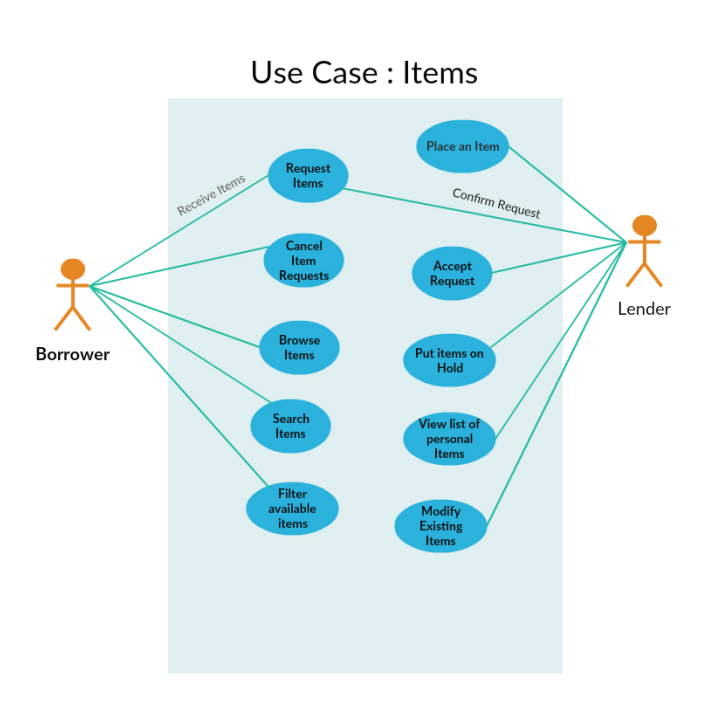
\includegraphics[width=0.9\textwidth]{usecase-Items.PNG}\hfill
  \caption{Users interaction with Items}\label{UseCase-Items}
\end{figure}

\subsection{User Registration \& Profile}
\begin{itemize}
\item \textbf{Sign up}: New User Registration
\item \textbf{Sign In} : Sign In for Existing Users
\item \textbf{View Notifications} : View Notifications regarding Item Requests.
\item \textbf{View Profile} : View one's profile.
\end{itemize}
\begin{figure}[H] 
  \centering
  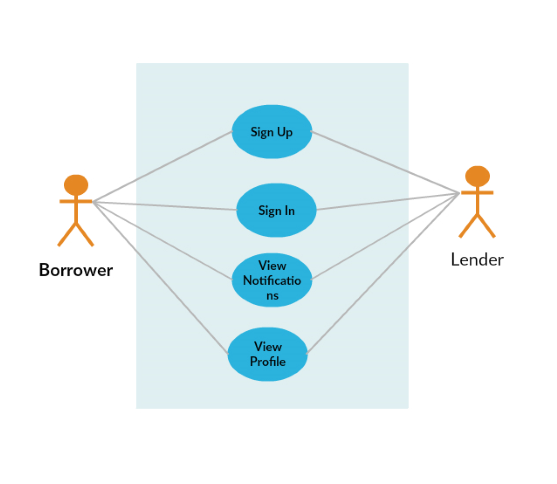
\includegraphics[width=0.9\textwidth]{usecase-Users.PNG}\hfill
  \caption{User Registration \& Profile}\label{Usecase-users}
\end{figure}



\section{ER model} All user-data and item information is stored in our MySQL database. It was also intended that the requests would be stored there as well. This however was, as previously mentioned, never implemented in the server-code or the front-end. The main entities of our System are : User, Items and Requests as shown in our ER Diagram generated by the backwards engineering function in MySQL workbench. Associated attributes are displayed within the entity blocks in the diagram.
\begin{itemize}
\item \textbf{Table Specification and Relationship Explanations}: The tables in our database are related and implemented in the following way : 
\begin{itemize}
\item \textbf{Requests} : A request in the requests table has a primary key that is the request id which uniquely identifies each request. There are also foreign keys to user, from user and requested item. Which all point to distinct rows in the users table and the items table. Specifying what item the request is regarding, what user sent the request and what user received the request.
\item \textbf{Items including tables such as Books, Tools, Etc} : All items stored in our database can be found in the items table. If it has a specific category it will also be stored in its respective table. For example, if the item is a book, it is stored in the items table and the books table with the same primary key. This means that adding additional categories is simply a matter of adding another table using the same primary key as the items table.
\item \textbf{Item subcategories tables such as book categories, tool categories etc}: These tables' primary keys are foreign keys in each category table. For example in the table Books there is a foreign key called book category id which in book categories specifies what that subcategory is called. A horror book is then stored in items, books and in books it is specified that the subcategory is Horror.
\item \textbf{Users} : The users table is fairly straight-forward. There the users' password, email and other information is stored. The password is encrypted before being stored in the table so that a if anyone gained access to the users table they would still not get hold of any sensitive information.
\end{itemize}

\end{itemize}
\begin{figure}[H] 
  \centering
  \includegraphics[width=0.9\textwidth]{database.png}\hfill
  \caption{ER Diagram}\label{ERDiagram}
\end{figure}

\section{System Implementation \& Evaluation}
\subsection{Implementation of functionality}
The functionalities we were able to implement were: 
\subsubsection{Add Items :} This page allows users to add items to the database. The user can select from a variety of categories, and each category contains their own subcategory. Each item is required a name and description, and depending on the subcategory, additional information can be added. The user can use their current location to add to the item, or they can type in an area and use that location. To ensure the right location is shown, a marker will be displayed on a map. The last part of add item is adding an image to go along with the item.
\begin{figure}[H] 
  \centering
  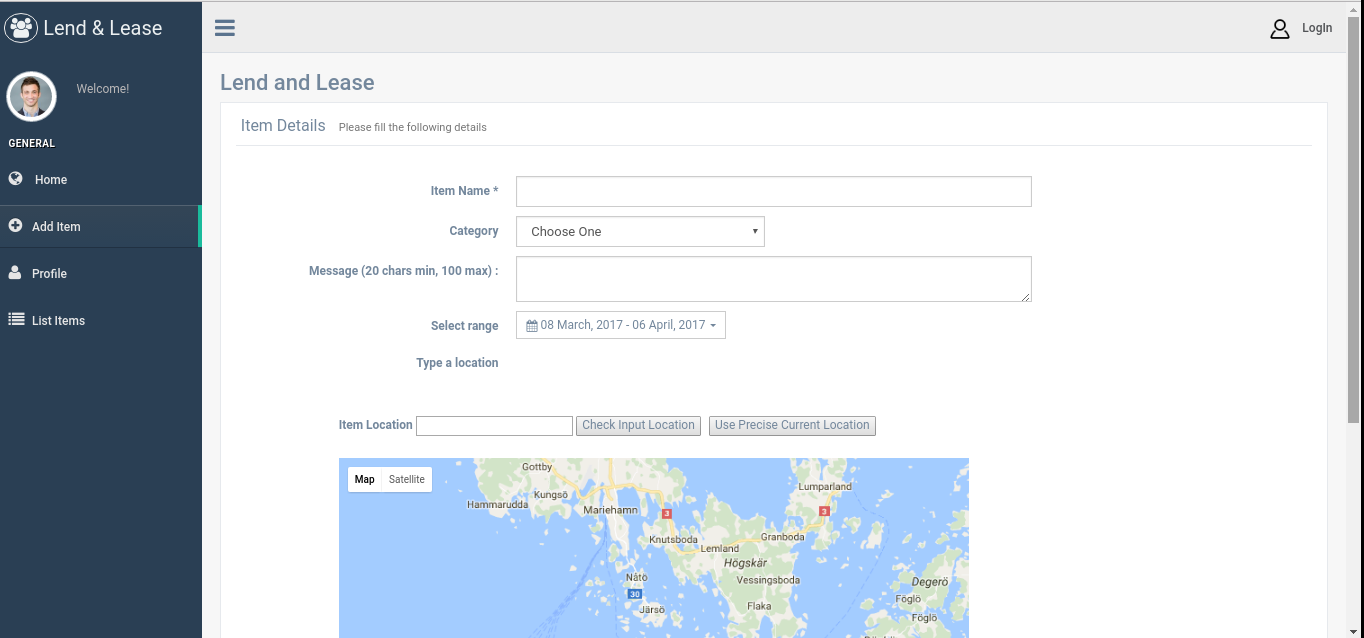
\includegraphics[width=0.9\textwidth]{addItems.PNG}\hfill
  \caption{Add items}\label{additems}
\end{figure}

\subsubsection{Profile :} To be able to view/ edit user's profile
\begin{figure}[H] 
  \centering
  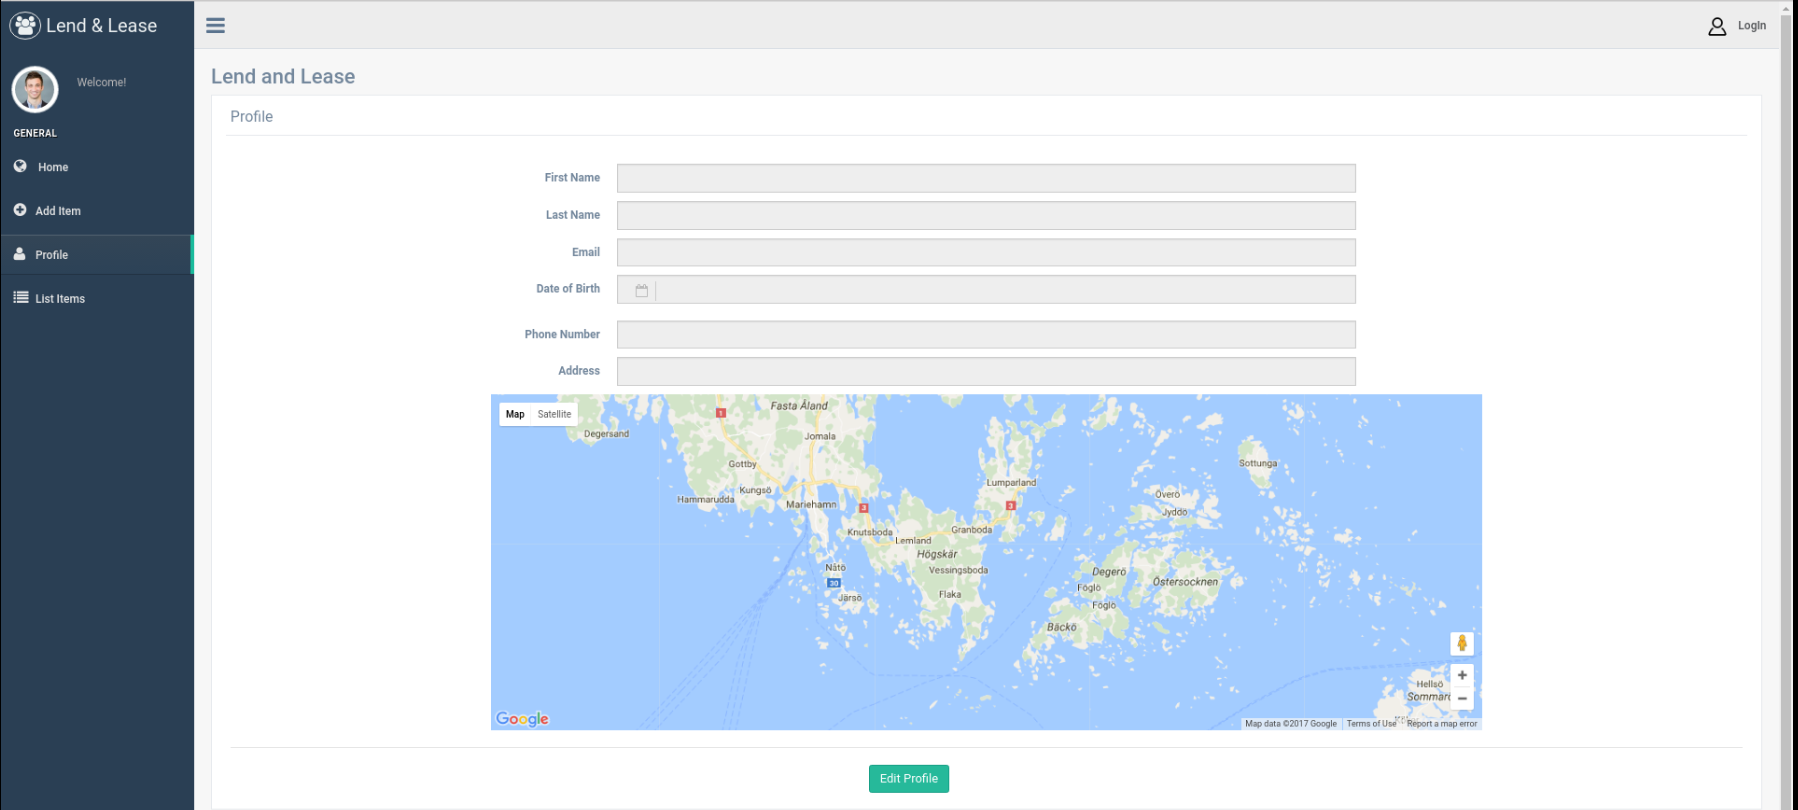
\includegraphics[width=0.9\textwidth]{profile.PNG}\hfill
  \caption{user Profile}\label{profile}
\end{figure}

\subsubsection{Maps :} Maps is available on the Home page as well as the add item page. On the map page, users will be prompted to access their current location, and can then browse the items in the area. In order to let users narrow down the amount of items, they can filter the items by category.
\begin{figure}[H] 
  \centering
  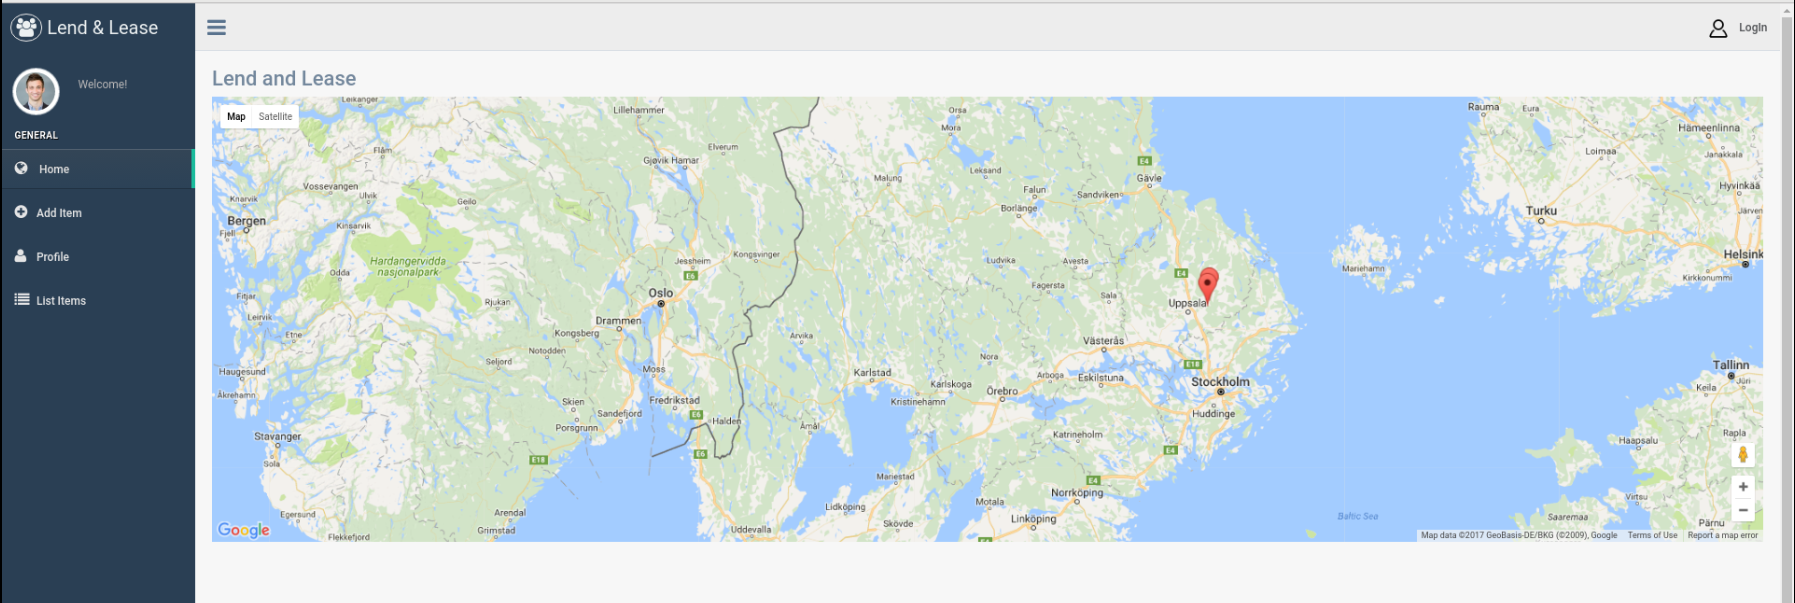
\includegraphics[width=0.9\textwidth]{home.PNG}\hfill
  \caption{Maps from Home page}\label{home}
\end{figure}
%screenshot

\subsection{Development Tools}
\begin{enumerate}
\item Github: For version control, we used Github to share code.
\item AngularJS : The Front-End of the system is using Google’s own framework - AngularJS. This is a perfect language for building dynamic web-applications and it fits perfectly with what we wanted our website to be. We wanted it to be a single-page application, with a sidebar for navigation and functionalities, leaving the center of the page to display information to the user and let him or her input their own information. 

\item NodeJS : The server built with NodeJS, using the express package to handle the HTTP requests and responses. What makes us satisfied with this choice is that NodeJS also has a package for communicating with MySQL databases which is our database of choice.

\item MySQL : For our database management we are using MySQL. The reason being that it is widely used and well-documented. Since AngularJS and NodeJS are somewhat new and poorly-documented we wanted something sturdy and trusted running the background if all else failed. 
\item node\_modules
\begin{itemize}
\item bcrypt-nodejs : used for encrypting user password. \cite{bcrypt}
\item express : used as a NodeJS web framework. \cite{express}
\item passport : used for Authentication. \cite{authentication}
\end{itemize}
\end{enumerate}

\section{Technical Problems Encountered } As we picked new languages and framework such as Angular and Node, it was difficult to get around with it. If we encountered some error, it was time consuming and annoying to find a fix for it. Also, there was not good enough documentation available to get a quick overview. 

\section{Testing and Security}
\subsection{Testing} We have not applied any kind of test-driven development during our progress of the project. After observing the usage of our finished product amongst users with different backgrounds, we have forged some personas which covers the typical user test cases. We have also performance tested the finished page with the framework 'siege'.
\subsubsection{Siege performance test result}
Below we can see a picture of our performance test during our siege.
It handled requests from 10 000 users with a fairly high increase in latency from the server. However, it did not cause the server to malfunction, which is a result we are satisfied with.
\begin{figure}[H] 
  \centering
  \includegraphics[width=1.0\textwidth]{siegetest.jpg}\hfill
  \caption{Screenshot from the siege test}\label{siegetest}
\end{figure}
\subsubsection{Persona 1}
Name: Gustav Farthinder \\
Age: 30 \\
Profession: IT consultant \\
Computer habit: High \\
\newline Gustav is a frequent user of pages like Blocket and Amazon. Suddenly, it occurs to him that he has several different
tools that are not used by him often. He does, however, not want to sell them as he might have a require them in
the future. Gustav comes up with the brilliant idea to lend them out when he's not using them. As he is highly involved
with the Internet and all of its possibilities, he searches for pages that supply this service.
He stumbles upon the page 'Lend and Lease' and feels that this serves his need perfectly!
As he enters the site, he immediately shares his location and sees a map with nearby objects that are up for lending and leasing.
He is not interested in loaning someones items, he wants to lend his own items out - and understands that he probably has to sign
up to be able to get in touch with possible loaners. He cannot find any "sign up"-button, so he presses Login.
He is taken to a login-page, which also has a button to sign up. He gets taken to the sign-up menu, where he fills in all his details
and adds a profile image of himself. After this, he is logged in and ready. He gets straight to his point and see the "add item" in the
left bar. He clicks it. He fills in all details about his lendable item and chooses his current location (as that is where the item is).
He continues to add the other items which he wants to lend out. After he is finished, he simply waits for people to send him requests.
Gustav is highly satisfied with his stay and loves the page.

\subsubsection{Persona 2}
Name: Jeanette 'Nettish' af Oxjärpe \\
Age: 27 \\
Profession: World famous painter \\
Computer habit: Below moderate \\
\newline Nettish is not too familiar how to handle the situation, now that she realizes that he has several brushes
which she does not frequently use. She wants to lend them out to people. After googling, she finds the page 'Lend and Lease'.
Nettish goes straight for finding how to put up her stuff for lending, without registering first. As there is no "register here"
button on the main page, the register button is on the login page. Nettish has trouble finding this, as she does not want to login,
she wants to register. She finally finds it and registers. Because she is filled with rage from his time wasted on not finding his way
to add an item, she misses that she has chosen the wrong location for her item when she has added it. Unfortunately, an edit item function has not yet been implemented. Nettish simply gives up and leaves the page, never to use it again. If she wanted to change it, she would
have had to delete her item and make a new entry, which is a quite  unnecessarily long way to go, for a pretty simple task.



\subsection{Security}
\subsubsection{Password Encryption} We used native NodeJS library called bcrypt for encrypting and storing users password which uses the latest Security Recommendation for cryptographic algorithm. \cite{bcrypt} 

\subsubsection{Session Implementation} Establish login session for user and destroy it when logged out. 

\section{Group Management}
We initially started with everyone trying to understand how to use node.js and AngularJS. One everyone knew the basics, we were to familiarize ourselves with the frameworks we planned to use. As the time went by, we had to get started on the project, and so we started dividing work as front end features and back end features.

As the project was being worked on, and after midterm presentation, we had to change the task division because not everyone was working at the same pace and the deadline was approaching. In the end, the final work division was done as two members on front-end, one on back-end, one on testing, and everyone working on the report. 

\section{Future Work}
The feature that we initially planned to implement but were not able to because of limited time was: 
\subsection{Chat Functionality} We initially planned to implement chat functionality in our App. This feature would enable requester and requestee to interact with one another and plan to exchange the requested item(s) they have.
\subsection{Premium Account}
This feature would be part of our payment plan, and would enable users with a premium account to avoid advertisements and be featred on the website.
\subsection{Enhanced Filtering}
The current filtering leaves a lot to be desired for users. With our planned enhanced filtering function, users would be able to type and search what they want instead of just narrowing down the categories.
\subsection{Location Loading}
With location loading, only items with locations in a close proximity to the user would be loaded, reducing loading time and improving speed for the user.
\subsection{Testing} We didn't have time to do testing in an efficient and correct way. Given more time, we would have liked to implement some testing frameworks such as mocha which is a javascript test frameworks that runs on nodejs. Also, we would have liked to use some standard testing methods like: QAcomplete, HP QC etc and create test cases and run them properly in parallel with development.

\section{Conclusion} 
The implementation we have so far is what we plan to deploy. As mentioned earlier, the languages \& frameworks we used were new so it was a bit of annoyance to pick it up. Also, because of limited time, we had to throw away some features we initially planned to work on. 

\section{Source Code}
\title{server.js}
\begin{lstlisting}[style=htmlcssjs]
// set up ======================================================================
// get all the tools we need
var express  = require('express');
var session  = require('express-session');
var cookieParser = require('cookie-parser');
var bodyParser = require('body-parser');
var morgan = require('morgan');
var path = require('path');
var mongoose = require('mongoose');
var mysql      = require('mysql');

var app      = express();
// var port     = process.env.PORT || 8080;
var port = 3000;
var passport = require('passport');
var flash    = require('connect-flash');

var fs = require('fs');
var util = require('util');


var connection = mysql.createConnection({
    host     : '198.211.126.133',
    user     : 'admin',
    password : 'password',
    database : 'lendandloan'
});

connection.connect();

// configuration ===============================================================
// connect to our database

require('./config/passport')(passport); // pass passport for configuration



// set up our express application
app.use(express.static(path.join(__dirname, 'public')));
app.use(bodyParser()); // get information from html forms
app.use(cookieParser()); // read cookies (needed for auth)
app.set('view engine', 'ejs'); // set up ejs for templating
// set up our express application
app.use(morgan('dev')); // log every request to the console
// required for passport
app.use(session({ secret: 'ilovescotchscotchyscotchscotch' })); // session secret
app.use(passport.initialize());
app.use(passport.session()); // persistent login sessions
app.use(flash()); // use connect-flash for flash messages stored in session
// routes ======================================================================
require('./app/routes.js')(app, passport); // load our routes and pass in our app and fully configured passport

// launch ======================================================================
app.listen(port);
console.log('The magic happens on port ' + port);
\end{lstlisting}

\title{config/database.js}
\begin{lstlisting}[style=htmlcssjs]
module.exports = {
    'connection': {
        'host': '198.211.126.133',
        'user': 'admin',
        'password': 'password'
    },
	'database': 'lendandloan',
    'users_table': 'users'
};
\end{lstlisting}\hspace*{\fill} \\

\title{config/passport.js}
\begin{lstlisting}[style=htmlcssjs]
// config/passport.js

// load all the things we need
var LocalStrategy = require('passport-local').Strategy;
var bcrypt = require('bcrypt-nodejs');

// methods ======================
// generating a hash
function generateHash(password) {
    return bcrypt.hashSync(password, bcrypt.genSaltSync(8), null);
};

// checking if password is valid
function validPassword(password, savedpass) {
    return bcrypt.compareSync(password, savedpass);
};


var mysql = require('mysql');

var connection = mysql.createConnection({
    host: '198.211.126.133',
    user: 'admin',
    password: 'password',
    database: 'lendandloan'
});

connection.connect();

// load up the user model
//var User            = require('../app/models/user');

// expose this function to our app using module.exports
module.exports = function (passport) {

    // =========================================================================
    // passport session setup ==================================================
    // =========================================================================
    // required for persistent login sessions
    // passport needs ability to serialize and unserialize users out of session


    // used to serialize the user for the session
    passport.serializeUser(function (user, done) {
        console.log("serialize User: " + JSON.stringify(user));
        console.log("serialize user id " + user.id);
        if(user.user_id == null){
            done(null, user.id);
          }
          else{
            done(null, user.user_id);
          }
    });
passport.deserializeUser(function(user, done) {
        done(null, user);
    });
    // =========================================================================
    // LOCAL SIGNUP ============================================================
    // =========================================================================
    // we are using named strategies since we have one for login and one for signup
    // by default, if there was no name, it would just be called 'local'

    passport.use('local-signup', new LocalStrategy({
            // by default, local strategy uses username and password, we will override with email
            usernameField: 'email',
            passwordField: 'password',
            passReqToCallback: true // allows us to pass back the entire request to the callback
        },
        function (req, email, password, done) {
            console.log("local-signup req: " + req);
            // asynchronous
            // User.findOne wont fire unless data is sent back
            process.nextTick(function () {

                // find a user whose email is the same as the forms email
                // we are checking to see if the user trying to login already exists
                connection.query("select * from users where email = '" + email + "'", function (err, rows) {
                    if (err)
                        return done(err);
                    if (rows.length > 0) {
                        return done(null, false, { message: 'That email already exists.' });
                    }
                    else {
                        var newUserMysql = new Object();
                        newUserMysql.email = email;
                        newUserMysql.password = generateHash(password);
                        newUserMysql.first_name = req.body.first_name;
                        newUserMysql.last_name = req.body.last_name;
                        newUserMysql.address = req.body.address;
                        newUserMysql.date_of_birth = req.body.date_of_birth;
                        newUserMysql.phone = req.body.phone;

                        var insertArray = [
                            newUserMysql.email,
                            newUserMysql.password,
                            newUserMysql.first_name,
                            newUserMysql.last_name,
                            newUserMysql.phone,
                            newUserMysql.date_of_birth,
                            newUserMysql.address
                        ]

//                        var insertQuery = "INSERT INTO users ( email, password, first_name, last_name, phone, dob, address ) values ('" + newUserMysql.email + "','" + newUserMysql.password + "')";
                        var insertQuery = "INSERT INTO users ( email, password, first_name, last_name, phone, dob, address ) values ( ? )";
                        connection.query(insertQuery, [insertArray], function (err, rows) {
                            if (err) {
                                console.log("Insertion failed");
                            }
                            newUserMysql.id = rows.insertId;

                            return done(null, newUserMysql);
                        });
                    }
                });
            })
        })
    );

    // =========================================================================
    // LOCAL LOGIN =============================================================
    // =========================================================================
    // we are using named strategies since we have one for login and one for signup
    // by default, if there was no name, it would just be called 'local'

    passport.use('local-login', new LocalStrategy({
            // by default, local strategy uses username and password, we will override with email
            usernameField: 'email',
            passwordField: 'password',
            passReqToCallback: true // allows us to pass back the entire request to the callback
        },
        function (req, email, password, done) { // callback with email and password from our form

            // find a user whose email is the same as the forms email
            // we are checking to see if the user trying to login already exists
            console.log("local-login email print : " + email);

            var queryString = "SELECT * FROM users WHERE email = '" + email + "'";

            console.log("local-login query string : " + queryString);

            connection.query(queryString, function (err, rows) {
                console.log("rows0 password print :" + rows[0].password);
                if (err)
                    return done(err);
                if (!rows.length) {
                    return done(null, false, req.flash('loginMessage', 'No user found.')); // req.flash is the way to set flashdata using connect-flash
                }

                // if the user is found but the password is wrong
                if (!validPassword(password, rows[0].password))
                    return done(null, false, req.flash('loginMessage', 'Oops! Wrong password.')); // create the loginMessage and save it to session as flashdata

                // all is well, return successful user
                return done(null, rows[0]);
            });

        })
    );



};
\end{lstlisting}\hspace*{\fill} \\

\title{public/app.js}
\begin{lstlisting}[style=htmlcssjs]
'use strict';

// Declare app level module which depends on views, and components
angular.module('myApp', [
    'ngRoute',
    'ngMap',
    'myApp.add_item',
    'myApp.items_list',
    'myApp.add_user',
    'myApp.login',
    'myApp.profile',
    'myApp.map'
]).
config(['$locationProvider', '$routeProvider', function ($locationProvider, $routeProvider) {
    $locationProvider.hashPrefix('!');
    $routeProvider.otherwise({redirectTo: '/map'});
}])
    .directive('file', function () {
        return {
            scope: {
                file: '='
            },
            link: function (scope, el, attrs) {
                el.bind('change', function (event) {
                    var file = event.target.files[0];
                    scope.file = file ? file : undefined;
                    scope.$apply();
                });
            }
        };
    })
    .run(function ($rootScope) {
    $rootScope.serverIP = 'http://localhost:3000';
});
\end{lstlisting}

\title{public/index.html}
\begin{lstlisting}[style=htmlcssjs]
\end{lstlisting}

\begin{thebibliography}{}	  
    
    \bibitem{bcrypt}
    bcrypt-nodejs,  A native JS bcrypt library for NodeJS, [Online].\\
    Available: https://www.npmjs.com/package/bcrypt-nodejs
    
    \bibitem{authentication}
    Authentication, "Easy Node Authentication", [Online]. \\
    Available: https://scotch.io/tutorials/easy-node-authentication-setup-and-local
    
    \bibitem{express}
    Express, "Web Framework for NodeJS", [Online]. \\
    Available: http://expressjs.com/
    
\end{thebibliography}

\end{document}